\chapter{Pruebas}

\section{Flujo de Arranque}
\begin{figure}[h]
\centering
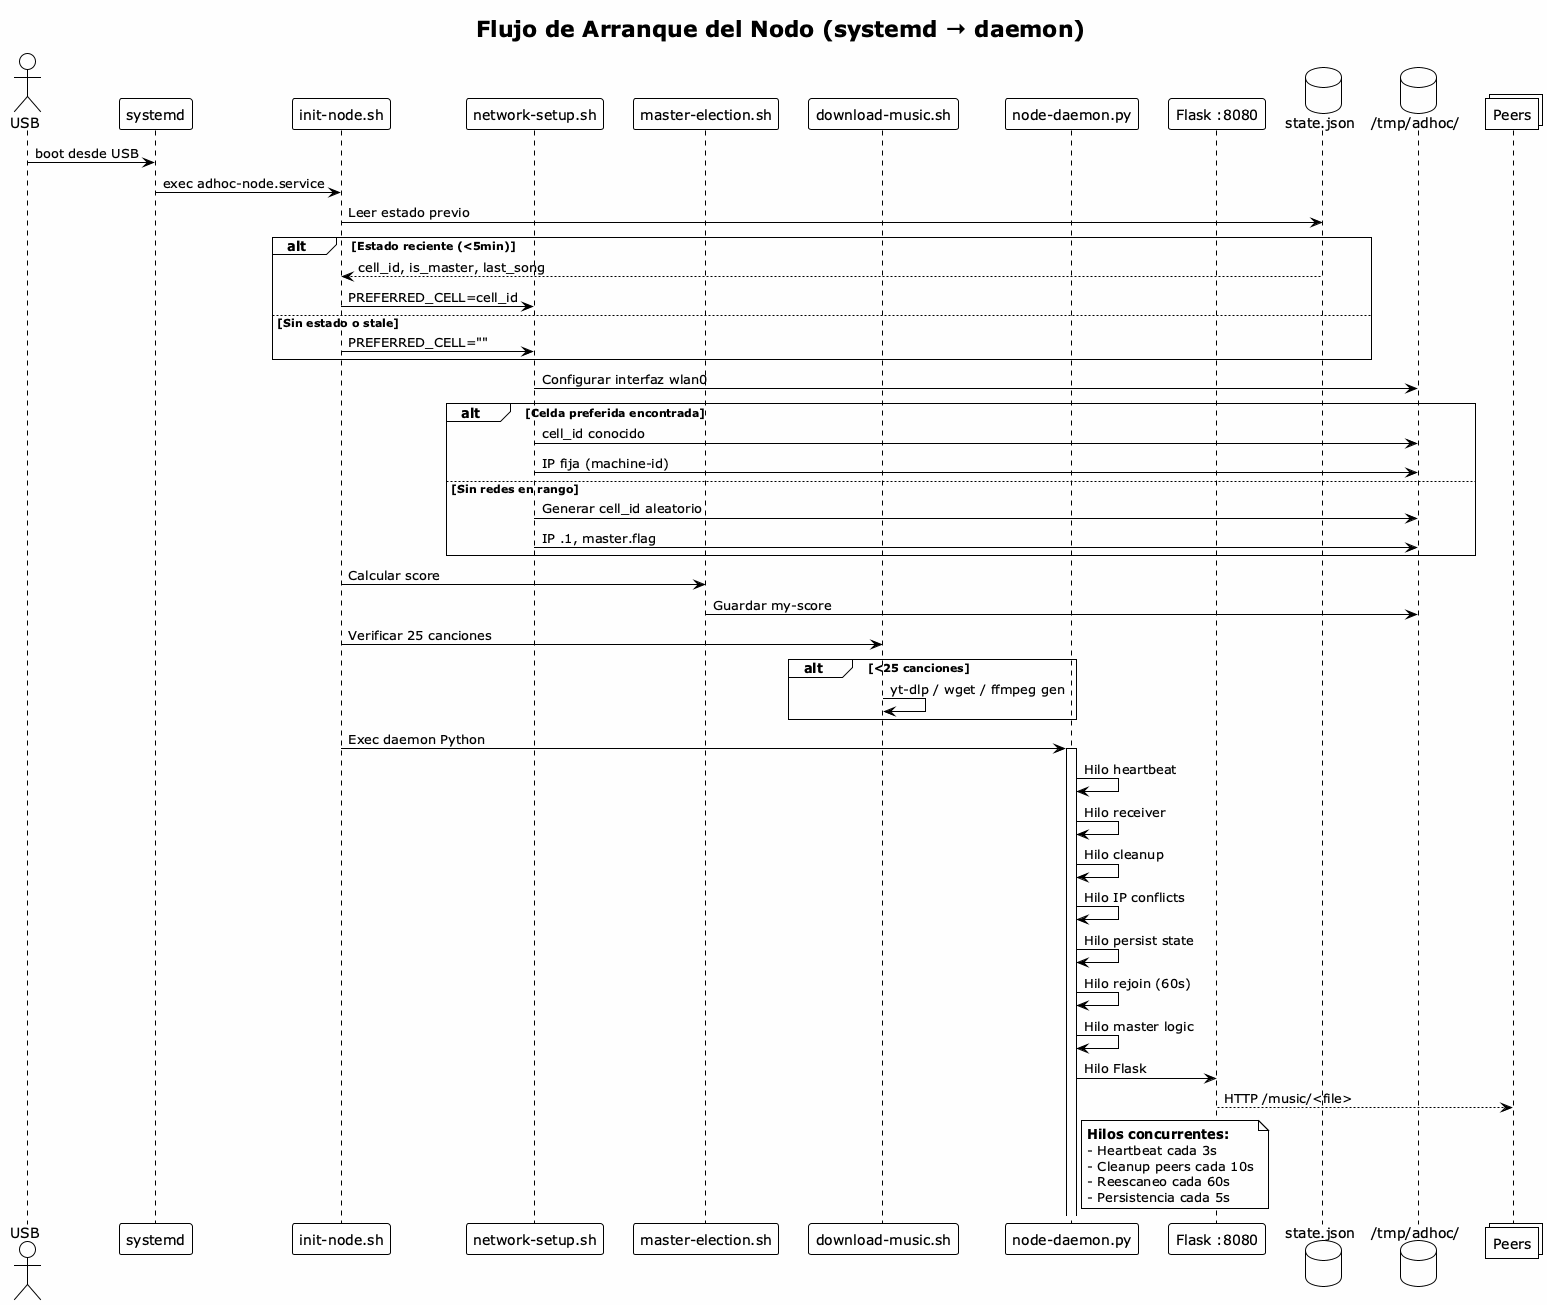
\includegraphics[width=\textwidth]{diagrams/boot-sequence.png}
\caption{Secuencia de arranque desde systemd hasta los hilos del daemon.}
\label{fig:boot}
\end{figure}

\section{Escenario 1: Un solo nodo}
El nodo arranca sin detectar redes, crea la celda IBSS, se auto-asigna IP \texttt{192.168.99.1} y comienza a streamar una canción aleatoria de sus 25 locales.

\section{Escenario 2: Dos nodos en rango}
El segundo nodo detecta la celda, se une con IP dinámica, recibe el heartbeat del primero, compara scores y asume rol de Cliente. Ambos reproducen la misma canción.

\section{Escenario 3: Pérdida de cobertura}
Al alejar el nodo Cliente fuera de rango, deja de recibir heartbeats. Tras timeout de 15s, limpia peers, no detecta red y crea su propia celda como nuevo Master.

\section{Escenario 4: Control externo}
Desde el panel web o vía \texttt{POST /api/force-song}, el Master cambia la canción en streaming a voluntad.
